\documentclass[Main]{subfiles}

\begin{document}


\section{Designprocess}
Dette afsnit indholder designet af systemet.

\subsection{Fjernbetjening}

Projektet skulle indeholde en sender, som kunne sende kommandoer til dronen.

\begin{figure}[H]
\centering
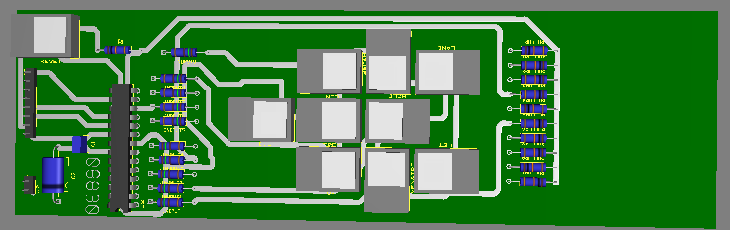
\includegraphics[width = 1 \textwidth]{3dUdenTal}
\caption{3D Figur af sender}
\label{Fig:3dUdenTal}
\end{figure}
\vspace{-20pt}

Senderen, som ses på figur \ref{Fig:3dUdenTal}, er bygget op med form som en fjernbetjening for, at det er muligt at betjene den med én hånd.
Fjernbetjeningen indeholder en µ-controller, en radiosender og knapper.
Knapperne giver brugeren mulighed for at vælge et program/kommando, der skal sendes til dronen. 
Når en knap bliver trykket ned, registrere µ-controlleren det og der genereres et frame med brugervalget. 
Dette frame bliver så sendt til radioen via SPI, hvorefter radioen får besked om at sende framet fra µ-controlleren.


\newpage
\subsection{4+1 View}
\begin{itemize}
\item Logical view: Sekvensdiagrammer af Use Cases, statisk klassediagram, klasse- og funktionsbeskrivelser.
\item Deployment view: Protokoller og kommunikation imellem forskellige enheder i projektet.
\item Process view: Samtidige processors kommunikation.
\item Implementation view: Beskrivelse af hvordan softwaren sættes op, kompileres, installation, software-eksekvering mm.
\end{itemize}

\subsubsection*{Logic View}

Fjernbetjeningen udgør den største del af de Use Cases beskrevet i kravspecifikationen\cite{Kravspec}.

Til udviklingen blev et lille scenarie (Figur \ref{Fig:Overview} optegnet og der kunne sættes nogle klassenavne på, som skulle forklare de forskellige hardware- og software-komponenter.

\begin{figure}[H]
\centering
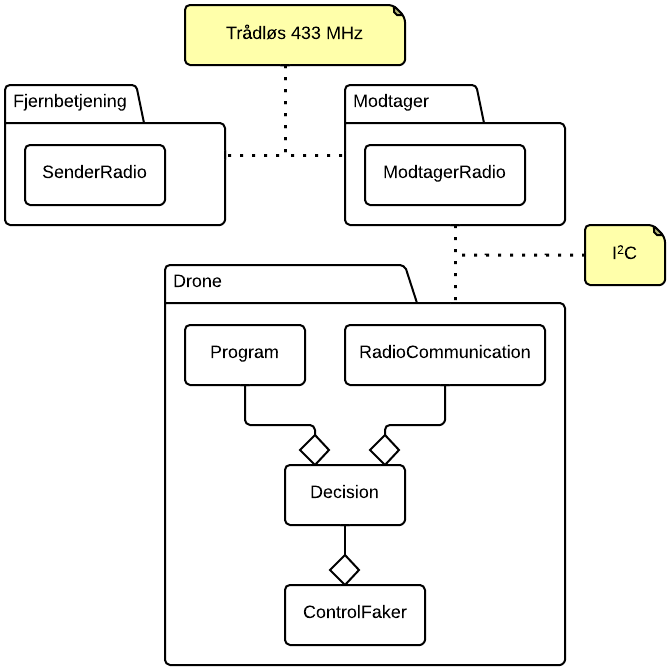
\includegraphics[width = 0.55 \textwidth]{Overview}
\caption{De første klasser.}
\label{Fig:Overview}
\end{figure}


Ved at analysere diagrammet yderligere med flere Use Cases, blev der optegnet flere klasser og til sidst var der et klassediagram. 
Fra klassediagrammet blev små sekvensdiagrammet herefter udtænkt, således forbindelsen fra fjernbetjeningen til dronen blev mere håndgribelig, som vist på Figur \ref{Fig:sendProgram}.


\begin{figure}[H]
\centering
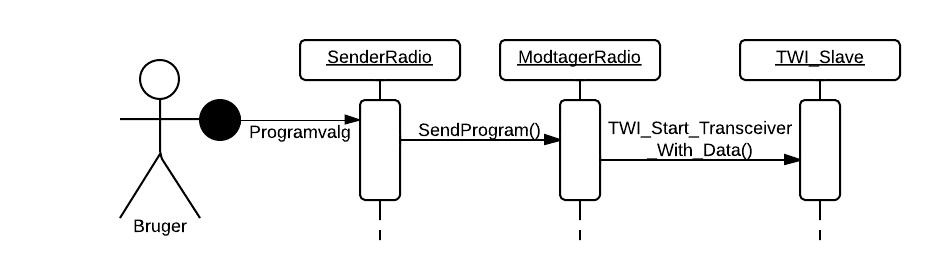
\includegraphics[width = 1.0 \textwidth]{SendProgram}
\caption{Sekvensdiagram fra fjernbetjening til drone.}
\label{Fig:sendProgram}
\end{figure}

\subsubsection*{Deployment View}

\begin{figure}[H]
\centering
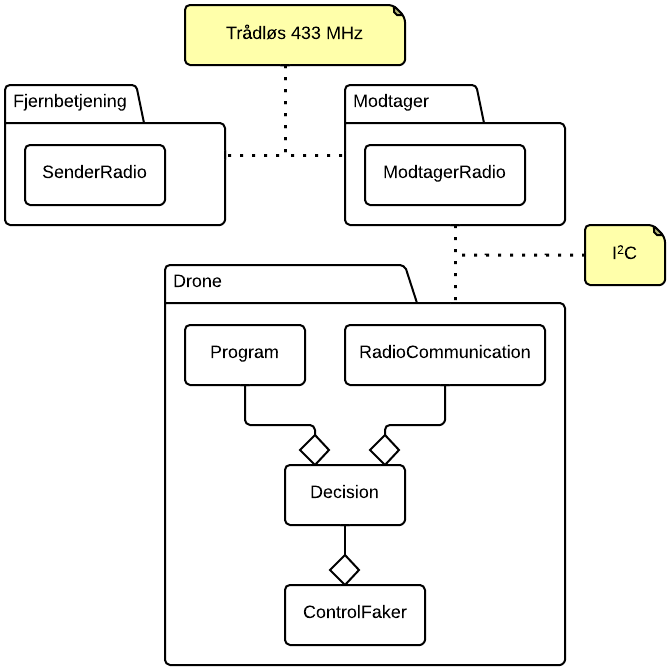
\includegraphics[width = 0.55 \textwidth]{Overview}
\caption{Intern kommunikation mellem enhederne.}
\label{Fig:Overview}
\end{figure}

Fjernbetjeningen sender et frame til dronen vha. det trådløse 433 MHz-signal, som opfanges af modtagerenheden.
Herefter bliver pakken lagt over i en output buffer til dronen. Dronen kan så hente denne pakke, når den har tid til det. 
Kommunikationen mellem dronen og modtageren sker gennem \itoc-protokollen, som vist på Figur \ref{Fig:Overview}.


\begin{figure}[H]
\centering
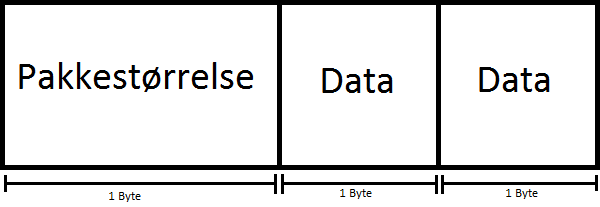
\includegraphics[width = 0.7 \textwidth]{PakkeUdenCrc}
\caption{Pakken fra fjernbetjening til drone.}
\label{Fig:PakkeUdenCrc}
\end{figure}

Pakken, der bliver sendt fra fjernbetjeningen over modtageren og til dronen, ser ud som vist på figur \ref{Fig:PakkeUdenCrc}.
Den første byte indeholder en indikator for, om det er et program der vælges.
Den anden byte er et nummer, som fortæller dronen hvilket program der skal køres.






\subsubsection*{Process View}

Projekt indeholder 3 processer, en på senderen, en på modtageren og en på dronen.
Processen på fjernbetjeningen snakker kun med radioen med normal SPI-kommunikation. 
Der er ikke problemer med overskrivning af data, der er ved at blive brugt af radioen.

Modtageren og dronen er to sideløbende processer, der snakker sammen.
Modtageren modtager et frame fra senderen, som sendes over \itoc til dronen.
For at sikre, at der ikke sker fejl, er der indlagt en sikkerhedsmekanisme på modtageren. 
Modtageren og dronen deler 2 byte mellem sig.

Når modtageren har en ny pakke til dronen, tjekker den først, om der er en \itoc-transmission i gang. 
Hvis dette ikke er tilfældet, bliver de nye data lagt ind i output bufferen. 
Næste gange dronen spørger på data, er disse tilgængelige.

\subsubsection*{Implementation View}
Koden til dronen, radiosenderen og radiomodtageren er skrevet i programmeringssproget C.

Der er tre dele at arbejde videre på:
\vspace{-20pt}
\begin{itemize}
\item Senderen.
\item Modtageren.
\item Dronen.
\end{itemize}

Det er muligt at videreudvikle på projektet.
En udførlig guide til hvordan man kommer i gang med det, kan findes i  designdokumentet\cite[Afsnit 2.4]{Design}.





\end{document}
